% Template inspired from https://github.com/hleskela/kth-master-thesis-templates/

\documentclass[12pt]{article}

% This is the preamble, load any packages you're going to use here
\usepackage{enumerate} % allows us to customize our lists
\usepackage{geometry} % to change margins
\usepackage{ragged2e} % provides \RaggedLeft
\usepackage{pdfpages}

\usepackage[backend=bibtex, natbib=true, style=numeric, sorting=none]{biblatex}
\addbibresource{bib.bib}

\begin{document}

\title{Specification and schedule}
\author{David Wobrock\ \texttt{wobrock@kth.se}}

\maketitle

\section*{Formalities}

\begin{itemize}
 \item Preliminary title: Design and development of image processing methods using spectral graph theory
 \item CSC Supervisor: Stefano Markidis (\texttt{markidis@kth.se})
 \item CSC Examiner: Erwin Laure (\texttt{erwinl@pdc.kth.se})
 \item Supervisor at workplace: Fr\'{e}d\'{e}ric Nataf (\texttt{nataf@ann.jussieu.fr})
\end{itemize}

\section*{Background \& Objective}

\subsection*{Description of the area within which the degree project is being carried out}

Spectral Graph Theory is a developing field with many applications through sociology, chemistry, biology, electrical engineering, computer science, topology and social networks such as Facebook or LinkedIn.
Network science studies the mathematical structure of the graphs that arise in these diverse fields, and the design, analysis, and applications of algorithms that compute with and on them.
For now days large graphs as the ones from social networks, memory requirements and computational times have become an issue.

Recent talks and research, especially at Google, have given that this graph theory can also be applied for new and fast image processing methods.

\subsection*{The principal's interest}

After working a lot with scientific computation in physics (finite element method among others), domain decomposition and high performance computing, it is an interesting topic to explore more possibilities of spectral graph theory \cite{ddm_nataf_2015}.
This is an important reason why delving into image processing is an application of interest.

\subsection*{Objective}

The objective of this project is to explore the usage of graph laplacian operator on images to compute filters, do segmentation, etc.
After applying these techniques on 2D images, they will also be used on 3D models.

\section*{Research Question \& Method}

\subsection*{The question that will be examined}

How to adapt the partial derivatives methods for matrices coming from graphs.

\subsection*{Specified problem definition}

Images can be interpreted as graphs, for which the Laplacian matrix can be used to build image processing tools.
These tools have been used for 2D images so far, but not yet for 3D models, which will be one of the biggest challenges of this degree project.

\subsection*{Examination method}

Smoothing, deblurring and sharpening 2D images are the first tasks \cite{modern_tour_2013} \cite{glide_2014}.
Image segmentation will be one the most interesting topics to dive into \cite{tolliver_spectral_2006} \cite{felzenszwalb_efficient_2004}.
They imply using approximation algorithms for the affinity matrix of the image graph, such as the Nystr\"om extension.
To build different filters, it will be necessary to use different kernel functions, but also try out different sampling techniques to approximate the image.
These algorithms will be executed on computers, not smartphone as Google is doing it, as it is not the aim of this project.
These algorithms will be implemented in Python, using the scientific modules numpy, scipy and matplotlib.

When the results are satisfying, we will explore the same techniques on 3D images.
The implementation details of these techniques will be studied once the 2D algorithms are acceptable.

\subsection*{Expected scientific results}

We first expect to master some image processing applications for 2D images and have them work properly and efficiently in order to apply the technique to 3D models.
We expect that the same techniques can be used for 3D models, by extending the current theorems, and have fast 3D model processing tools when using HPC.

\section*{Evaluation \& News Value}

\subsection*{Evaluation}

The degree project has been fulfilled once we achieve 3D models processing in a reasonable time.
2D images can be efficiently processed on smartphones according to \cite{siam_slides_2016} \cite{glide_2014}, which gives an idea on the achievable goals for 3D image processing.
However, 2D algorithms will just be implemented as prototypes on a computer.

\subsection*{The work's innovation/news value}

The added value of this project is new and fast processing techniques for 3D models.

\section*{Pilot Study}

\subsection*{Description of the literature studies}

The literature study will focus firstly on spectral graph theory and graph laplacian operator.
I will explicitly mention some specific topics about spectral graph theory and image processing.

This presentation \cite{siam_slides_2016} will serve as base for the pre-study, including its references.

\section*{Conditions \& Schedule}

List of resources: \\
\begin{itemize}
 \item hardware: the supplied laptop (running Ubuntu, 3GB RAM, Intel i3 processor), a server for light computations (24 cores, 64GB RAM) and a server heavier and parallel computations (160 cores, 640GB shared RAM)
 \item software: Python (Numpy), \LaTeX
 \item people: an available supervisor and friends
 \item perseverance: because it's tough to write a master thesis
\end{itemize}

\subsection*{Collaboration with the principal}

The collaboration with the supervisor happens at least once a week with a meeting.
More meetings are to be expected if particular help is needed at some point.
The whole research team is meeting once every two weeks.

\section*{Schedule}

As an early planning of the degree project, it is expected that the first part of understanding and implementing what exists for 2D images can take put to two months.
Then three months are planned to apply this to 3D images.
And finally one month for writing and completing the report and presentation.

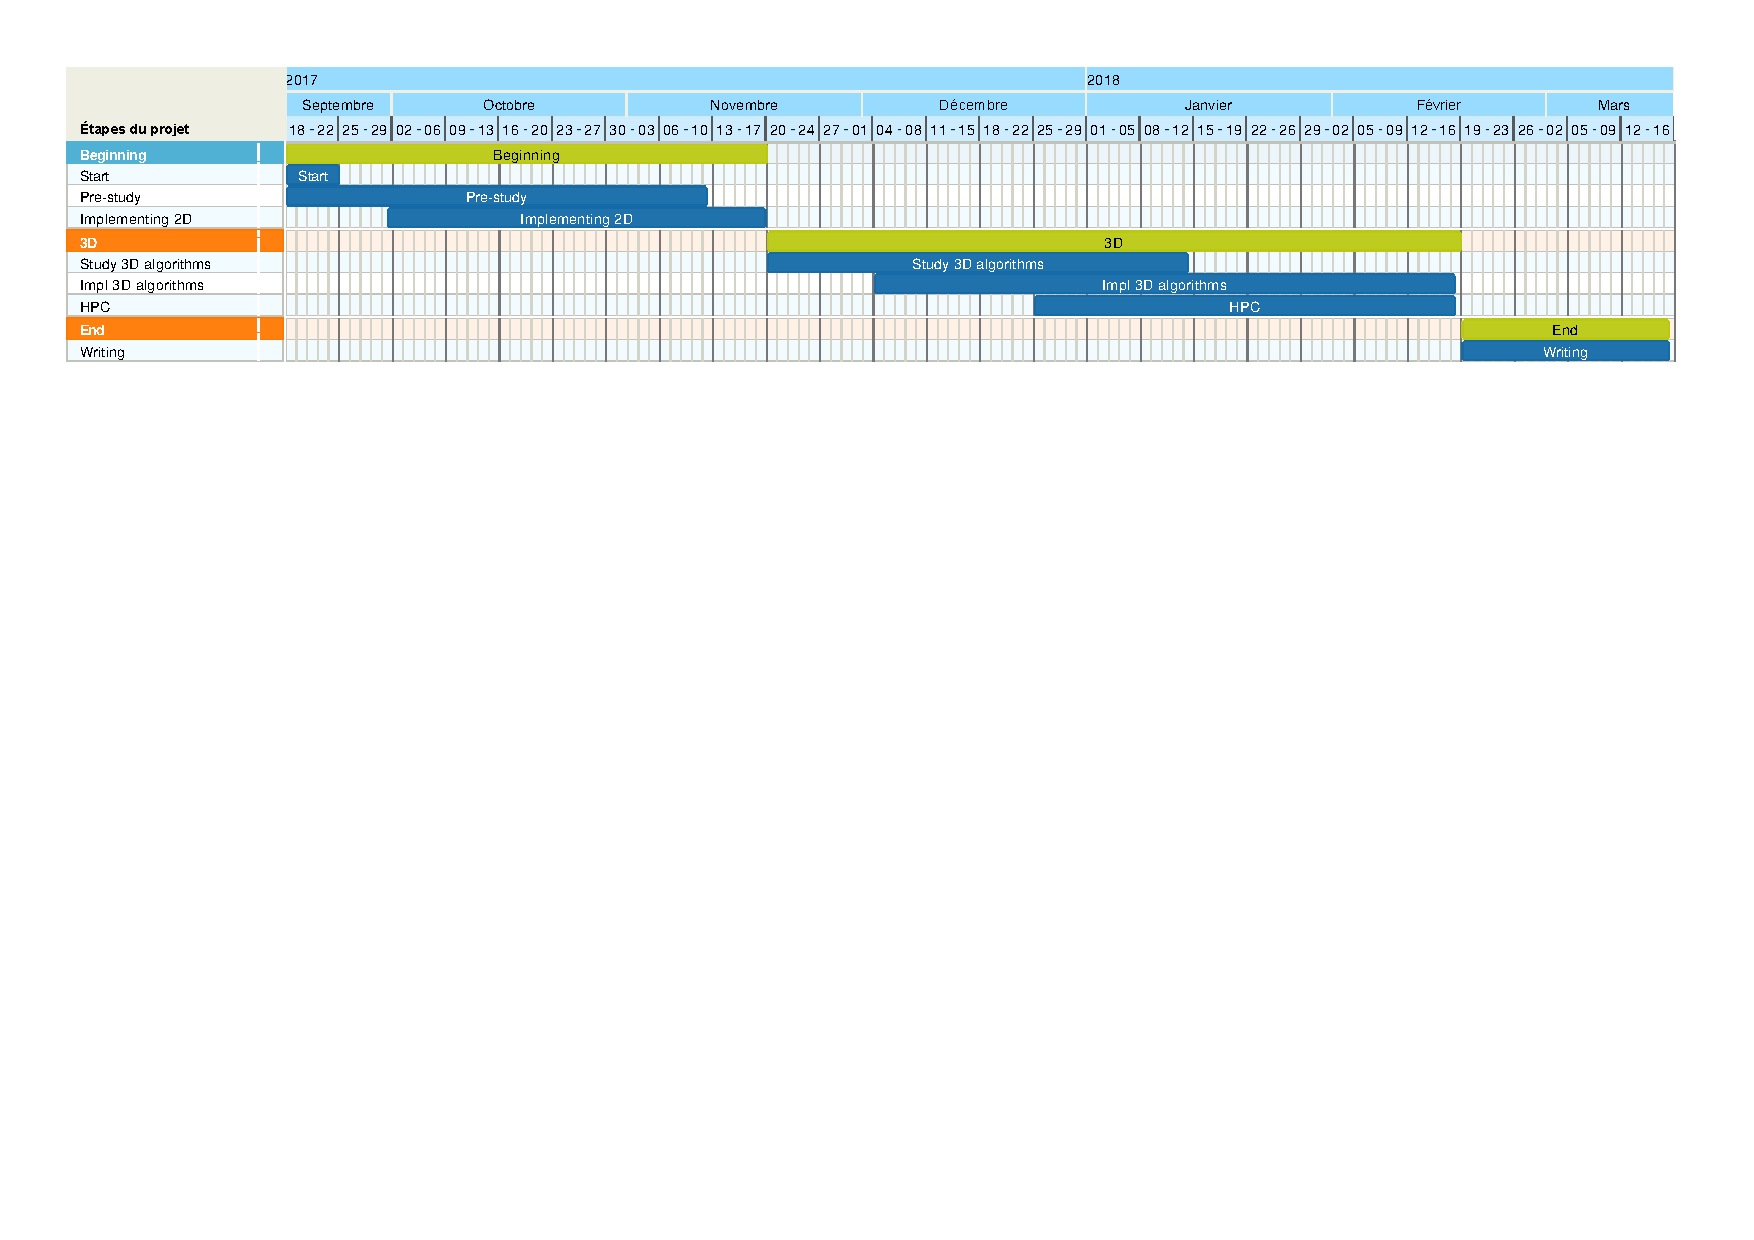
\includepdf[landscape=true]{schedule.pdf}

\printbibliography

\end{document}
